\documentclass[a4paper, oneside, 12pt]{scrartcl}

\usepackage[english, german]{babel}
\usepackage[utf8]{inputenc}

\usepackage{
  eurosym,
  listings,
  scrhack,
  pdfpages,
  lscape,
  graphicx,
  rotating,
  hyperref,
  tabu,
  longtable,
  datetime
}

\hypersetup{
  colorlinks = true,
  linkcolor = black,
  urlcolor = blue
}

\definecolor{backcolour}{rgb}{0.90, 0.90, 0.90}

\lstdefinestyle{default}{
  backgroundcolor = \color{backcolour},
  breaklines = true
  basicstyle = \tiny,
  columns = fullflexible
}

\lstset{style = default}

\title{boneserver}
\subtitle{Installations- und Betriebsanleitung}
\author{Caspar Friedrich}
\date{\today}

\begin{document}

%Titlepage
\maketitle

%Table of contents
\tableofcontents

\newpage

%Sections
\section{Hardware}
Dieses Handbuch ist für den \textbf{BeagleBone Black Revision A5C} (im Folgenden kurz als BeagleBone bezeichnet) geschrieben und getestet. Sofern nachfolgende oder vorangegangen Revisionen zu dieser kompatibel sind, sollte die Installation aber dennoch problemlos möglich sein.

\section{Installation}
Als Betriebssystem wird \href{http://archlinuxarm.org/}{Arch Linux ARM} verwendet, eine Portierung von Arch Linux für ARM-Prozessoren. Arch Linux ARM stellt auch ein spezielles package repository zur Verfügung.

\subsection{SD-Karte vorbereiten}
Auf der Homepage von Arch Linux ARM gibt es eine Installationsanleitung, die laufend aktualisiert wird. Die folgende Anleitung ist daher im Wesentlichen eine Übersetzung ausgehend von einem Linux als Host-System. Stattdessen kann auch die mitgelieferte {\AA}ngström Distribution verwendet werden, die mit dem BeagleBone ausgeliefert wird.

\paragraph{Voraussetzungen} sind die Softwarepakete \textit{dosfstools} und \textit{wget} sowie root-Rechte und eine Micro SD-Karte mit mindestens 2GB Speicherkapazität.

\begin{enumerate}

\item Finden Sie zunächst heraus, welcher Laufwerkspfad der vorgesehenen SD-Karte enspricht. Meist \textit{/dev/sd[a, b, ...]} oder \textit{/dev/mmcblk[0, 1, ...]}.

{\paragraph{\color{red} ACHTUNG} \textbf{\color{red} Überprüfen Sie Laufwerkspfade genau, bevor Sie mit der Installation beginnen, da sonst irreparable Schäden am Host-System auftreten können!}}

\item Starten Sie \emph{fdisk}, um die SD-Karte zu formatieren:

\begin{lstlisting}
fdisk /dev/sdX
\end{lstlisting}

\item Erstellen Sie eine neue Partitionstabelle und die nötigen Partitionen.\\
Dazu geben Sie nacheinander die folgenden Kommandos ein (jeweils mit \textit{enter} bestätigen):

\begin{longtabu} to \textwidth {
	X[1]
    X[3]}
\textbf{Kommando} & \textbf{Funktion}\\
o & Erzeugt eine neue Partitionstabelle\\
n, p, 1 & Erzeugt eine neue (n), primäre (p), erste (1) Partition\\
\textit{enter} & Bestätigt den Default-Wert für den ersten Sektor\\
+64M & +64M als letzten Sektor setzt die Partitionsgröße auf 64MByte\\
t, e & Ändert den Partitionstyp auf \textit{W95 FAT16 (LBA)}\\
a, 1 & Setzt das boot flag der ersten Partition (je nach \emph{fdisk}-Version wird die erste Partition automatisch ausgewählt, da nur eine zur Verfügung steht)\\
n, p, 2 & Erzeugt eine neue (n), primäre (p), zweite (2) Partition\\
2x \textit{enter} & Setzt die Default-Werte für den ersten und letzten Sektor der Partition\\
w & Schreibt Änderungen in die Partitonstabelle
\end{longtabu}

\item Formatieren der ersten Partition:

\begin{lstlisting}
mkfs.vfat -F 16 /dev/sdX1
\end{lstlisting}

\item Formatieren der zweiten Partition:

\begin{lstlisting}
mkfs.ext4 /dev/sdX2
\end{lstlisting}

\item Laden Sie den \textit{bootloader tarball} herunter und entpacken Sie ihn auf die erste Partition der SD-Karte:

\begin{lstlisting}
wget http://archlinuxarm.org/os/omap/BeagleBone-bootloader.tar.gz
mkdir boot
mount /dev/sdX1 boot
tar -xvf BeagleBone-bootloader.tar.gz -C boot
sync && umount boot
\end{lstlisting}

\item Laden Sie den \textit{rootfs tarball} herunter und entpacken Sie ihn auf die zweite Partition der SD-Karte (hierzu müssen Sie als \textit{root} eingeloggt sein, \emph{sudo} reicht in diesem Fall nicht):

\begin{lstlisting}
wget http://archlinuxarm.org/os/ArchLinuxARM-am33x-latest.tar.gz
mkdir root
mount /dev/sdX2 root
tar -xf ArchLinuxARM-am33x-latest.tar.gz -C root
sync && umount root
\end{lstlisting}

\item Stecken Sie die SD-Karte in den BeagleBone und halten Sie die Taste S2 gedrückt, um von der SD-Karte zu booten, während Sie die Power-Taste (S3) betätigen.\\
Wenn das System gestartet ist, können Sie sich auf der Kommandozeile oder via \emph{ssh} einloggen.\\

Benutzernahme/Passwort lautet \textbf{root/root}.

\end{enumerate}

Aus Sicherheitsgründen sollten Sie nach dem Systemstart als erstes das root-Passwort ändern:

\begin{lstlisting}
passwd root
\end{lstlisting}

Da man sich, außer zu Wartungszwecken, nicht am System anmelden muss, kann auf die Erstellung eines regulären Benutzers verzichtet werden.


\subsection{Installation im internen Speicher}

\paragraph{Hinweis} Der BeagleBone hat zwar eine eingebaute Uhr allerdings keine Batterie. Nach einem Neustart kann es daher passieren, dass die interne Uhr auf den Default-Wert zurück gesetzt wird. Überprüfen Sie mittels \emph{date} die aktuelle Systemzeit und aktualisieren diese gegebenenfalls via \texttt{ntpdate -u pool.ntp.org}

\begin{enumerate}
\item Um Arch Linux direkt auf der eMMC zu installieren, aktualisieren Sie zunächst das eben gestartete System und installieren die Pakete \emph{wget}, \emph{dosfstools} und \emph{ntp}.

\begin{lstlisting}
pacman -Syu wget dosfstools ntp
\end{lstlisting}

Das Paket \emph{ntp} stellt hierbei das Programm \emph{ntpdate} zur Verfügung (s. O.).

\item Der interne Speicher ist bereits korrekt partitioniert, folgen Sie daher nur den Schritten 4 bis 7. Die Partionen sind \textit{mmcblk1p1} bzw. \textit{mmcblk1p2} (s. O.).

\item Fahren Sie das System herunter und warten Sie bis alle LEDs erloschen sind.

\item Entfernen Sie die SD-Karte und starten das System erneut.
\end{enumerate}


\subsection{boneserver installieren}

\paragraph{Repository klonen}
\textit{boneserver} ist via \href{https://github.com/XMrVertigoX}{GitHub}\footnote{https://github.com/XMrVertigoX} verfügbar. Führen Sie dazu zunächt ein Systemupdate durch, um alle Pakete auf den neusten Stand zu bringen und installieren Sie das Paket \emph{git}. Anschließend klonen Sie das Repository nach \texttt{/opt}.

\begin{lstlisting}
pacman -Syu git
git -C /opt clone https://github.com/XMrVertigoX/boneserver.git
\end{lstlisting}

\paragraph{Installationsskript ausführen} Im root-Verzeichnis des Repositories befindet sich ein Skript, welches die weitere Installtaion übernimmt. Wechseln Sie dazu in das Verzeichniss und führen das Installationsskript aus.

\begin{lstlisting}
cd /opt/boneserver
./install.sh
\end{lstlisting}

Hierbei werden alle erforderlichen Pakete und Module installiert, die Konfigurationsdateien verlinkt sowie die Daemons installiert und gestartet.\\

Wenn das Skript fehlerfrei durchgelaufen ist, wird der BeagleBone automatisch neu gestartet und die Installation ist abgeschlossen.

\section{Betrieb}
Für die Verwendung des Webinterface wird eine Netzwerkverbindung zum BeagleBone und ein Webbrowser\footnote{Das Webinterface verwendet \emph{JQuery} in der Version 2.1.1, aktuelle webbrowser sollten hier keine Probleme bereiten. Ansonsten kann die Homepage von JQuery konsultiert werden: \url{http://jquery.com/browser-support/}} mit aktiviertem JavaScript vorausgesetzt.


\subsection{Netzwerkverbindung herstellen}

\paragraph{Hinweis:} Die Standardkonfiguration des BeagleBone sieht den Betrieb mit einem DHCP-Server vor. Sollte dies nicht gewünscht oder möglich sein, kann über die üblichen Wege eine statische IP eingestellt werden. Anleitungen hierzu findet man im Internet.\\

Steht ein DNS-Server zur Verfügung, kann der BeagleBone über seinen Hostname erreicht werden, standardmäßig \textit{boneserver}. Ansonsten finden Sie zunächst heraus, welche IP dem BeagleBone zugewiesen wurde. Hierfür kann entweder die Routing-Tabelle des DHCP-Servers konsultiert werden oder in der Kommandozeile via \emph{ip} die aktuelle Addresse der einzelnen Netzwerkadapter abgerufen werden \mbox{(Abb. \ref{fig:getBeagleBoneIP})}.

\begin{figure}[ht]
	\centering
	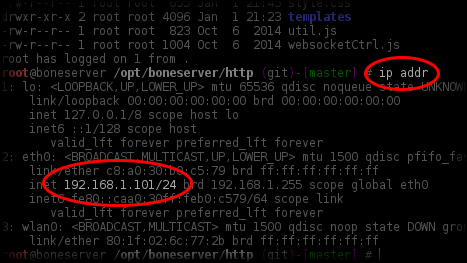
\includegraphics[width=0.7\textwidth]{betriebsanleitung/images/getBeagleBoneIP.png}
	\caption{IP des BeagleBone abrufen}
	\label{fig:getBeagleBoneIP}
\end{figure}


\subsection{Webinterface aufrufen}
Das Webinterface kann einfach über DNS-Namen oder die IP im Webbrowser aufgerufen werden. Ist die Verbindung hergestellt, wird dies durch einen grünen Haken rechts in der Titelleiste angezeigt \mbox{(Abb. \ref{fig:mainWindowConnected})} und die Steuerelemente werden generiert.
Sollte die Verbindung einmal unterbrochen werden, wechselt dieser Haken in ein rotes Kreuz. In diesem Fall kann die Seite neu geladen werden, eventuelle Konfigurationen bleiben erhalten.

\paragraph{Passwortschutz} Um unbefugten Zugriff zu verhindern ist das Webinterface passwortgeschützt. Wenn Sie dieses Passwort änderen möchten, generieren Sie zunächst einen neuen Datensatz z. B. mit dem \href{http://jesin.tk/tools/htdigest-generator-tool/}{\textit{htdigest Generator Tool}}\footnote{ \url{http://jesin.tk/tools/htdigest-generator-tool/}} und tragen die Zugangsdaten in die Datei \textit{config/lighttpd/lighttpd.user} ein. Die Default Login-Daten sind \textbf{admin/AgG7KgW4}

\begin{figure}[ht] 
	\centering
	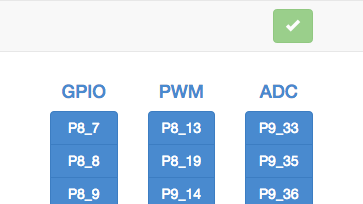
\includegraphics[]{betriebsanleitung/images/mainWindowConnected.png}
	\caption{Webinterface verbunden}
	\label{fig:mainWindowConnected}
\end{figure}

\paragraph{Hinweis} Das Webinterface kann immer nur von einem Fenster aus aufgerufen werden. Es kann daher passieren, dass bei einem schnellen Fensterwechsel oder Neuladen der Seite die Verbindung nicht sofort hergestellt wird. In dem Fall einfach ein paar (Milli-)Sekunden warten, bis die Verbindung wieder frei ist.


\subsection{Bedienelemente}
Wie in \mbox{Abbildung \ref{fig:webinterface}} gezeigt hat die Weboberfläche des boneserver drei Anzeigegruppen:

\begin{itemize}
\item[\textbf{1}] \textbf{Verbindungsanzeige}\\
zeigt grün, wenn die Steuereinheit verbunden ist und rot, wenn die Verbindung unterbrochen ist (vgl. Abb. \ref{fig:mainWindowConnected}).
\item[\textbf{2}] \textbf{Bedienfelder} für digitale I/O, PWM und AIN\\
Hier findet die tatsächliche Bedienung der GPIO statt. Es gibt drei Sektionen jeweils für digitale I/O, PWM und AIN. Die Bedienung der verschiedenen Kacheln wird weiter unten beschrieben.
\item[\textbf{3}] \textbf{Anzeigenschalter} für die einzelnen Pins\\
Hier können einzelne Kacheln ein- bzw. ausgeblendet werden, um die Oberfläche übersichtlicher zu gestalten und an die Arbeitsumgebung anzupassen. Diese Funktion dient ausschließlich der Übersicht, eine ausgeblendete Kachel bleibt weiterhin aktiv und kann jederzeit wieder eingeblendet werden. Diese Einstellungen bleiben auch nach einem Neustart erhalten.
\end{itemize}

\begin{figure}[ht] 
	\centering
	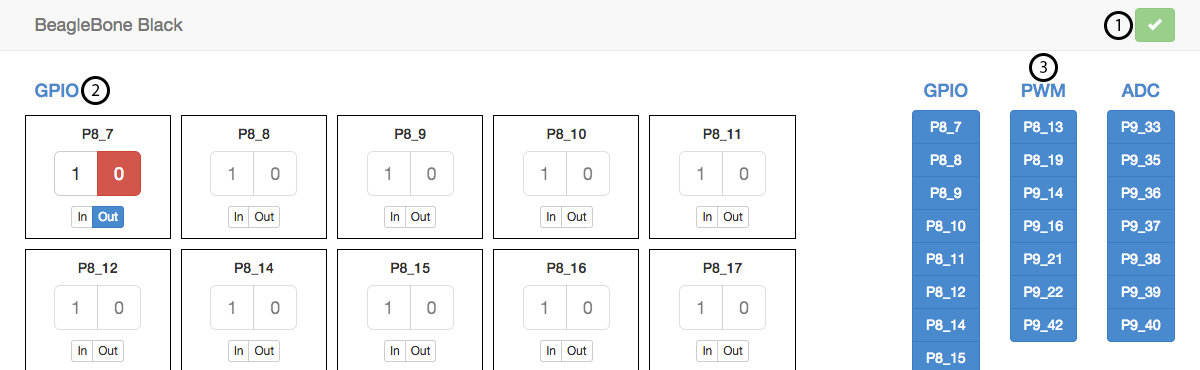
\includegraphics[width=1.0\textwidth]{betriebsanleitung/images/controlElements.png}
	\caption{Weboberfläche}
	\label{fig:webinterface}
\end{figure}

\subsubsection{Digitale In- und Outputs}
Die Konfigurationskachel \mbox{(Abb. \ref{fig:mainWindowGPIODisabled})} für digitale I/O besteht aus zwei Schaltern: Betriebsrichtung und logic level.

\paragraph{Betriebsrichtung} Jeder digitale I/O kann entweder als Input oder als Output konfiguriert werden. Dazu kann über den Wahlschalter \textbf{In/Out} jederzeit das Gewüschte ausgewählt werden.

\paragraph{logic level} Wenn der GPIO als Output konfiguriert ist, kann hier mittels der beiden Schaltflächen, \textbf{1} und \textbf{0}, ein logisches high und ein logisches low eingestellt werden. Ist der GPIO als Input konfiguriert, ist diese Schaltfläche deaktiviert und zeigt stattdessen den Status der Leitung an. Die GPIO sind mit einem internen Pulldown-Widerstand beschaltet.

\begin{figure}[ht] 
	\centering
	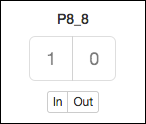
\includegraphics[]{betriebsanleitung/images/mainWindowGPIODisabled.png}
	\caption{Deaktivierte GPIO-Kachel}
	\label{fig:mainWindowGPIODisabled}
\end{figure}


\subsubsection{Pulsbreitenmodulation (PWM)}
Mit Hilfe der PWM-Kacheln \mbox{(Abb. \ref{fig:mainWindowPWMDisabled})} werden die GPIO konfiguriert, über die eine Pulsbreitenmodulation möglich ist.\\

Der BeagleBone stellt insgesamt sieben PWM-Ausgänge mit insgesamt vier Timern zur Verfügung. Dabei teilen sich jeweils die Pinne P8\_13/19, P9\_14/16 und P9\_21/22 einen Timer. P9\_42 hat einen exklusiven Timer. Die Ausgänge mit einem gemeinsamen Timer haben dementsprechend immer dieselbe Frequenz und laufen absolut synchron.\\

Über die Buttons \textbf{Enable} und \textbf{Disable} kann der jeweilige Ausgang aktiviert bzw. deaktiviert werden. Wenn ein PWM-Ausgang deaktiviert wird, werden alle Einstellungen bezüglich Frequenz und Pulsbreite gelöscht!

\paragraph{Periodendauer} Über das Eingabefeld \textbf{Period} wird die Periodendauer in Nanosekunden (ns) eingestellt. Kleinster Wert ist hier 1 ns ($\hat{=}$ 1GHz) und der größte $10^9$ ns (= 1s $\hat{=}$ 1Hz).

\paragraph{Pulsbreite} Über das Eingabefeld \textbf{Duty} wird die Pulsbreite zwischen 0 und 1 eingestellt. Hier wird intern ebenfalls mit Nanosekunden gearbeitet, daher kann der tatsächliche Wert zusätzliche Nachkommastellen bekommen.

\begin{figure}[ht] 
	\centering
	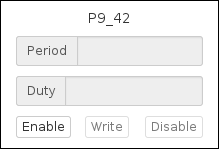
\includegraphics[]{betriebsanleitung/images/mainWindowPWMDisabled.png}
	\caption{Deaktivierte PWM-Kachel}
	\label{fig:mainWindowPWMDisabled}
\end{figure}

Mit \textbf{Write} werden die Parameter abgesendet.

\paragraph{Hinweis} Der Linux Kernel arbeitet intern mit ganzen Nanosekunden, daher ist die Genauigkeit der Pulsbreite von der Höhe der Periodendauer anhängig.

\paragraph{Bug:} Wenn beide Ausgänge eines PWM-Generators aktiviert sind, lässt sich die Frequenz bei keinem der beiden ändern. Wenn bei einem der beiden PWMs die Frequenz zunächst geändert wurde, kann der zweite Ausgang nicht verwendet werden. Dies ist ein Problem der im Hintergrund verwendeten device tree overlays und wird in nachfolgenden Versionen der Bibliothek behoben.


\subsubsection{Analoge Inputs}
Mit diesen Kacheln \mbox{(Abb. \ref{fig:mainWindowADC})} werden die Analog/Digital-Converter gesteuert und die Eingangswerte in einem Echtzeitdiagramm angezeigt.\\

Mit den Tasten \textbf{Start} und \textbf{Stop} wird die Aufzeichnung gestartet bzw. gestoppt. Parallel zur Anzeige werden die Messdaten aufgezeichnet. Über \textbf{Download} können sie als CSV-Datei heruntergeladen werden.\\

Die Taste \textbf{Delete} löscht die zu diesem Eingang gespeicherte Messreihe um Speicherplatz frei zu machen.

\paragraph{\color{red} ACHTUNG} \textbf{\color{red} Laden sie Messreihen immer herunter, bevor Sie sie löschen, die Messdaten sind sonst unwiederbringlich verloren!}

\begin{figure}[ht] 
	\centering
	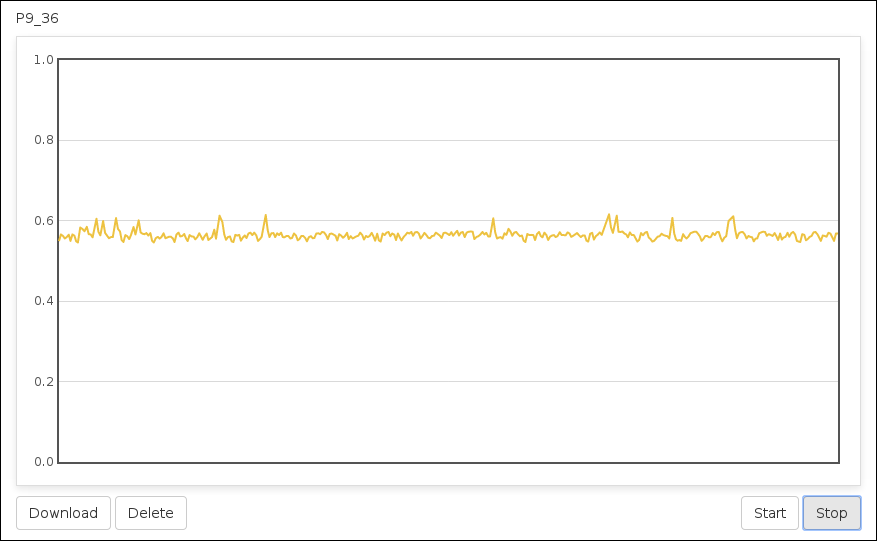
\includegraphics[width=0.9\textwidth]{betriebsanleitung/images/mainWindowAIN.png}
	\caption{ADC-Kachel}
	\label{fig:mainWindowADC}
\end{figure}


\subsection{Erweiterte Einstellungen}
Zusätzlich gibt es die Möglichkeit, über die Datei \textit{settings.json} im root-Verzeichnis des boneserver weitere Einstellungen vorzunehmen. Ist keine solche Datei vorhanden, wird die mitgelieferte \textit{settings-default.json} verwendet. Die Parameter überschreiben die Default-Werte, es müssen daher nur abweichende Werte eingetragen werden.\\

Die Datei ist eine JSON\footnote{JavaScript Object Notation (JSON) ist in der RFC 7159 beschrieben}-Datei in der folgende Parameter eingestellt werden können:\\

\begin{longtabu} to \textwidth {X[1] X[3]}
    
  \textbf{host} & IP des WebSocket Servers\newline
  Dieser Wert sollte nicht verändert werden, da sonst der WebSocket Server möglicherweise nicht mehr über das Webinterface erreichbar ist.\newline
  \textit{default: localhost}\\
  \textbf{port} & Netzwerk-Port des WebSocket Servers\newline
  Dieser Wert sollte nicht verändert werden, da der WebSocket Server sonst nicht mehr über das Webinterface erreichbar ist.\newline
  \textit{default: 8081}\\
  \textbf{gpioSampleRate} & Abtastrate der digitalen Inputs in Millisekunden\newline
  Angegeben wird die Zeit zwischen den Abfragen. Dieser Wert kann erhöht werden um die System- und Netzwerklast zu verringern.\newline
  \textit{default: 100}\\
  \textbf{adcSampleRate} & Abtastrate der analogen Inputs in Millisekunden\newline
  Angegeben wird die Zeit zwischen den Abfragen. Dieser Wert kann erhöht werden, um die System- und Netzwerklast sowie um die Menge der erhobenen Messwerte zu verringern. Dies ermöglicht bei gleichem Speicherplatz längere Messreihen.\newline
  \textit{default: 10}\\
  \textbf{dataLocation} & Speicherpfad für die Messdaten der ADC\newline
  Hier kann ein alternativer Pfad zur Speicherung der Messdaten eintragen werden. Es können auch externe Speicherorte wie z. B. USB-Sticks, USB-Festplatten oder Netzlaufwerke verwendet werden.\newline
  \textit{default: ./data}
\end{longtabu}

\paragraph{Hinweis} Die Datei \textit{settings-default.json} sollte nicht verändert werden, da sonst nicht ohne weiteres ein Update durchgfeührt werden kann.

\section{Wartung}
Als Wartungssystem wird die oben erstellte SD-Karte verwendet. Dazu starten Sie den BeagleBone von der SD-Karte und führen die oben beschriebenen Installationsschritte aus.\\

Die Paketverwaltung unter Arch Linux heißt \emph{pacman}, über sie können neue Pakete aus den Repositories installiert bzw. aktualisiert werden.\\
Ein kurzer Auszug aus der man-page zu den hier verwendeten Parametern:\\

Synopsis: \texttt{pacman <operation> [options] [targets]}\\

\begin{longtabu} to \textwidth {X[1] X[4]}

\textbf{Parameter} & \textbf{Beschreibung}\\
\textit{Operations}\\
-S, -\--sync & Synchronize packages. Packages are installed directly from the ftp servers, including all dependencies required to run the packages.\\

\textit{Sync Options}\\
-c, -\--clean & Remove packages that are no longer installed from the cache as well as currently unused sync databases to free up disk space.\\
-u, -\--sysupgrade & Upgrades all packages that are out of date.\\
-y, -\--refresh & Download a fresh copy of the master package list from the server(s) [...]. This should typically be used each time you use \textit{-u} or \textit{-\--sysupgrade}.\\
\end{longtabu}


\subsection{Backup}
Da der interne Speicher des BeagleBone \glqq nur\grqq ~2GB beträgt, kann ohne größerem Zeitaufwand ein komplettes Speicherabbild erstellt werden. Dies hat den Vorteil, dass es beim Einspielen von Backups keine Kompatibilitätsprobleme auftreten können.

Im Ordner \glqq scripts\grqq ~sind zwei shell-Skripte, die diesen Vorgang vereinfachen: \textit{backup.sh} und \textit{restore.sh}. Dabei wird das Image automatisch mit \emph{gzip} komprimiert, um Speicherplatz zu sparen. Das restore-Skript verwendet diese Dateien, um das Speicherabbild wieder auf den BeagleBone zu kopieren.\\

Sollte die SD-Karte nicht genügend Speicherplatz zur Verfügung stellen, kann ein USB-Stick verwendet werden. Dazu einfach das USB-Laufwerk einhängen\footnote{Anleitungen hierzu gibt es in ausreichender Zahl im Internet} und das entsprechende Verzeichnis als Zielverzeichnis angeben.

\begin{lstlisting}
backup.sh [Zielverzeichnis]
\end{lstlisting}

Das Zielverzeichnis ist dabei optional. Wenn kein Parameter übergeben wird, erstellt das Skript automatisch eine Datei in der Form \textit{backup-[timestamp].img.gz} im aktuellen Verzeichnis.

\begin{lstlisting}
restore.sh <Quelldatei>
\end{lstlisting}

Die Quelldatei ist hier Vorraussetzung.

\paragraph{Hinweis} Die Skripte verwenden intern \emph{dd}, um eine bitweise Kopie der eMMC des BeagleBone anzufertigen. Zudem ist die Quelle bzw. das Ziel immer \textit{/dev/mmcblk1}. Daher sollten diese Skripte nur von der SD-Karte aus verwendet werden.


\subsection{System aktualisieren}
Arch Linux verwendet die Rolling-Release-Technik, ein System, bei dem es keine großen Upgrades des gesamten Betriebssystems gibt, sondern die Softwarepakete einzeln laufend aktualisiert werden.\\
Trotz umfangreicher Tests der Pakete kann es zu Inkompatibilitäten kommen. Dies ist wahrscheinlicher, je mehr Pakete gleichzeitig aktualisiert werden. Daher sollte, gerade wenn das System nur selten aktualisiert wird, vorher ein vollständiges Backup angelegt werden (s. o.).\\

Das System kann jederzeit via \emph{pacman} aktualisiert werden:

\begin{lstlisting}
pacman -Syu
\end{lstlisting}


\subsection{boneserver aktualisieren}
Um die boneserver-Software zu aktualisieren, aktualisieren Sie zunächt Ihre Kopie des git Repositories und führen das Installationsskript erneut aus. Pakete, die bereits installiert sind, werden dabei nicht erneut installiert.

\begin{lstlisting}
cd /opt/boneserver
git pull
./install.sh
\end{lstlisting}


\subsection{System bereinigen}
\emph{pacman} speichert bei jeder Aktualisierung die alten Pakete, um jederzeit auf frühere Versionen zurückgreifen zu können. Je nach Häufigkeit der Aktualisierung und gemessen an der Kapazität der eMMC, kann der Speicher schnell knapp werden. Daher können alte Pakete via pacman in zwei Stufen gelöscht werden:

\begin{lstlisting}
pacman -Sc 
\end{lstlisting}

Löscht alle Paketversionen nicht mehr installierter Pakete und

\begin{lstlisting}
pacman -Scc
\end{lstlisting}

löscht sämtliche nicht verwendeten Pakete.


\end{document}